% This is ''sig-alternate.tex'' V2.0 May 2012
% This file should be compiled with V2.5 of '\'sig-alternate.cls'' May 2012
%
% This example file demonstrates the use of the \'sig-alternate.cls'
% V2.5 LaTeX2e document class file. It is for those submitting
% articles to ACM Conference Proceedings WHO DO NOT WISH TO
% STRICTLY ADHERE TO THE SIGS (PUBS-BOARD-ENDORSED) STYLE.
% The \'sig-alternate.cls' file will produce a similar-looking,
% albeit, 'tighter' paper resulting in, invariably, fewer pages.

\documentclass{sig-alternate}
\sloppy
\usepackage{paralist}
\usepackage{url}

\begin{document}
%
% --- Author Metadata here ---
\conferenceinfo{WIPSCE}{2015 London, UK}
\CopyrightYear{2015} % Allows default copyright year (20XX) to be over-ridden - IF NEED BE.
%\crdata{0-12345-67-8/90/01}  % Allows default copyright data (0-89791-88-6/97/05) to be over-ridden - IF NEED BE.
% --- End of Author Metadata ---

\title{Technocamps: A Decade of Supporting\\Computer Science Education in Wales}

\numberofauthors{2}
\author{
% 1st. author
\alignauthor
Tom Crick\\
\affaddr{Department of Computing}\\
\affaddr{Cardiff Metropolitan University, UK}\\
\affaddr{tcrick@cardiffmet.ac.uk}
% 2nd. author
\alignauthor
Faron Moller\\
\affaddr{Department of Computer Science}\\
\affaddr{Swansea University, UK}\\
\affaddr{F.G.Moller@swansea.ac.uk}\\
}

\maketitle

\begin{abstract}
Computing education in the UK over the past five years has undergone
significant scrutiny and upheaval. In September 2014, we saw the
implementation of a new computing curriculum in England, alongside
significant investment in the professional development of teachers in
Scotland. However, in Wales, numerous political and geographical
issues have hindered any substantive educational policy or curriculum
reform for computing education. This is despite the fact that Wales
was addressing the failings of computing education in schools since at
least 2003 through Technocamps, a pan-Wales university-based schools
outreach programme. In this paper we outline the history (and
pre-history) of Technocamps; explain the devolved nature of education
in the UK focusing on Wales with its specific issues and challenges;
and present data both in support of university engagement and
intervention as well as the positive effect this intervention is
having.
\end{abstract}

% A category with the (minimum) three required fields
\category{K.3.2}{Computers \& Education}{Computer and Information Science Education}[Computer Science Education]
\category{K.4.1}{Computers And Society}{Public Policy Issues}
\keywords{Computer Science Education; High School; Teachers}

\section{Introduction}
% taken from TOCE pitch from 2013
In the early 1980s, the BBC Micro was introduced to schools throughout
Britain for the \emph{BBC Computer Literacy Project}.
Before long they were in 80\% of UK classrooms~\cite{vasko:1986}.
By encouraging young learners to experiment with computers, a generation
of creative (and computational) talent was spawned. Applications in
the UK to study computer science at university hit a peak, and
computer science graduates changed the world as they helped computers
come to dominate every aspect of our lives.

Fast forward 30 years and the situation could not be any more
different. The computer is no longer a novelty. Children now typically
spend more time at home in front of a computer screen than a TV screen, but
like the TV, their interest is restricted to using the computer, not
in experimenting with it. Computer studies in school -- now called
Information and Communication Technology (ICT) -- has evolved into IT
studies with an emphasis on digital literacy and office skills --
significantly more mundane than the social networking and gaming for
which the pupils use their home computers. A full 66\% of ICT teachers
in the UK do not have a relevant qualification but have slipped into
the role of ICT teacher simply by being sufficiently digitally
literate~\cite{RoyalSoc:2012}.
The situation is worse in Wales, where this figure rises to
75\%~\cite{GTCW:2008}.
Applications to
study computer science at university slumped in the early part of the
millenium -- especially amongst females -- and
many of those who started a university computer science degree course
found themselves dropping out during the first year as they entered
unaware of what computer science is and what studying it entails.

In the early 2000s, the Department of Computer Science at Swansea University
started looking into ways to address this issue.
Unfortunately, attempts to reach out to teachers in local schools
faced great resistence, due naturally to their lack of confidence
in anything more complicated than using a desktop package.

As an alternative route into schools, Swansea University created
\emph{Technocamps} in 2003, an outreach programme which brings groups
of school children to the University campus for day-long workshops based on
selected computational themes to inform them what computing is about,
followed-up by support in setting up
extracurricular clubs -- \emph{Technoclubs} -- in the schools.
Technocamps proved very successful as a local initiative, with many
students studying computer science at Swansea University claiming to be
influenced by Technocamps activities.

In 2010, based on empirical data
regarding its effect on school children's attitudes towards computing
-- as well as their teachers -- Swansea University was awarded
\pounds 3.9 million funding towards a \pounds 6 million four-year project
(with the remaining \pounds 2.1 million
generated through University match funding)
by the Welsh Government under the EU's European Social
Fund (ESF) Convergence Programme to run Technocamps as a pan-Wales
project with regional hubs at
the Universities of Aberystwyth, Bangor and
South Wales Glamorgan.
(Technocamps hubs have subsequently been set up at most of the remaining
major Universities in Wales, specifically Cardiff University,
Cardiff Metropolitan University, and Glynd\^wr University Wrexham.)
Though focusing on the children, Technocamps also provides ``Technoteach"
events aimed at up-skilling ICT teachers in Welsh schools.
Technocamps has since provided computing-related activities and resources
for tens of thousands of young people across Wales, as well as interacting
with hundreds of teachers at hundreds of the nation's schools.

Technocamps is not alone in exploring solutions to a
perceived problem in Computer Science education.
In particular, in 2008 the
Computing At School (CAS) organisation was formed, and its current
membership of over 18,000 teachers and computing professionals
work hard to promote the teaching of computing at school in England.
However, whilst great changes have taken place in England
due in no small part to CAS lobbying,
the CAS effect is relatively unnoticed in Wales,
and the rapid changes pushed through in England
are in many ways resisted by Welsh Government.

Wales is a devolved nation within the United Kingdom, with its own
elected national government fully responsible for its education system.
At the 2012 Annual Technocamps Teachers' Conference,
the Welsh Government's Minister for Education and Skills
publicly acknowledged the importance of computer science education;
noted that he is a key supporter of Technocamps;
and expressed understanding of the wider educational and
socio-economic impact that the government can make with reform in Wales.
However, with only 5\% of the population of England and with its distinct
geographical and socio-cultural challenges, Wales presents
a variety of unique challenges in addressing curriculum reform.

In this paper, we will describe the backdrop to Technocamps and why it
was created in the way it was (Section 2); explain the devolved nature
of education in the UK focusing on Wales with its specific challenges
and issues (Section 3); and present data both in support of university
intervention as well as the positive effect this intervention is
having (Section 4).  We finish with a consideration of the challenges
remaining in Welsh education (Section 5).

\section{Computing Education in Wales and England}

In the 1980s, Computer Studies was a popular subject
in schools across Britain. The ubiquitous presence, in schools and homes,
of the popular BBC Micro -- which was useful for little else than
writing programs in BASIC -- saw a large proportion
of school children learning the fundamentals of program design
in a curriculum which included a variety of complementary
topics such as hardware, software, Boolean logic
and binary number representation~\cite{Doyle:1988}.

By the 1990s, however, the emergence of pre-installed software
packages -- specifically word processors and spreadsheet programs --
meant that computers were no longer predominantly machines that needed
to be programmed in order to do anything useful or interesting.  Less
and less time was being spent in the Computer Studies classroom on
thinking about and writing programs, as basic digital literacy became
regarded as its key skill.  However, as interest in viewing the
computer as a creative tool waned in favour of using it for more
mundane tasks, various problems were being created, which were
highlighted in two independent enquiries in 1997: the McKinsey
Report~\cite{McKinsey:1997} and the Stevenson
Report~\cite{Stevenson:1997}.  Both reports concluded that Information
Technology in UK schools was in a primitive state and in need of
attention and major investment.  In line with the Stevenson
Report, Computer Studies evolved into a new
subject whose name was coined in that Report: Information and
Communication Technology (ICT).  Over the decade starting in 1997, the
UK Government invested over \pounds3.5 billion in ICT in schools
through various initiatives such as the National Grid for Learning
(NGfL) and the New Opportunities Fund (NOF)~\cite{Doughty:2006}.

By 2000, then, ICT had permeated both primary and secondary school
curricula.  The emphasis was on developing the children's IT skills
and digital literacy in an honest attempt to address the increasing
need for digital literacy amongst the public.  However, despite
enormous government-funded ICT initiatives, various reports throughout
the decade identified problems with implementing government policy on
ICT educational
reform~\cite{OpieFukuyo:2000,Ofsted:2001,Ofsted:2002,Ofsted:2004,
Loveless:2005}.  Younie~\cite{Younie:2006} summarises the problems
identified by these reports into five key areas, three being
management and the other two being: teacher training and competence;
and impact on pedagogy.

A decade later, a report by the Royal Society~\cite{RoyalSoc:2012}
makes the very same observations.  The report noted that ICT suffers
from a poor reputation amongst pupils and other stakeholders, who
consider it dull and unchallenging and hence a low-value discipline,
especially compared to other STEM subjects.  With ICT embedded across
the primary school curriculum, secondary school pupils find ICT in
secondary school unstimulating.  The Wolf report~\cite{Wolf:2011}
further notes that the undemanding nature of ICT qualifications in
secondary schools is readily exploited by the schools: due to a high
league table weighting associated with vocational qualifications,
easily-achieved high results in ICT offer a welcome boost to a
school's league table position.  Furthermore, as ICT is typically
presented by schools as their computer science offering, students who
might otherwise enjoy studying computer science are left with a
positive distaste for what they are led to believe is computer science.

\subsection{Technocamps at Swansea University}
As experienced by other Universities,
the numbers of students enrolling in Computer Science
at Swansea University increased through the end
of the millenium due to the dot-com boom.
However, as depicted in Figure~\ref{fig:numbers},
\begin{figure}
  \centering
  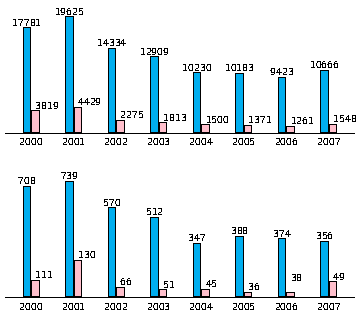
\includegraphics[width=0.9\columnwidth]{images/numbers.png}
  \caption{Applications to University Computer Science programmes
           in the UK (top) and Wales (bottom), males (blue) and females (pink).
           (Source: UCAS, Universities and Colleges Admissions Service,
            https://www.ucas.com)}
  \label{fig:numbers}
\end{figure}
the numbers peaked and was followed by
a steady five-year decline, dropping more than 40\% during that time,
with the worst effect on the already-dwindling numbers
of female students.
Even at its peak, more than a third of students who
started a computer science degree programme left
the programme before their second year of study,
citing a mistaken understanding of the subject
as their reason for leaving.

In an attempt to address this anomaly,
the Computer Science Department reached out
to local secondary school ICT teachers,
inviting them to meetings at the University,
and offering to visit schools to discuss
the subject with the teachers and to give
motivational talks to students.
Indeed, the Department was invited every year to
a number of English schools to present such talks
to school children making University choices.
However, interest was more than absent:
there was positive resistance to the Department
giving talks to their University seekers;
such activity was typically characterised as merely pitching for students.
In reality, for reasons explained later
which did not apply to English teachers,
teachers in Wales were generally feeling over-burdoned and
uninterested in exploring any perceptions
of inadequacy in their curriculum delivery.

As it proved impossible to influence schools and their ICT teachers directly,
Technocamps was created in 2003 to promote computing amongst their pupils.
This was a programme of fun and engaging interactive computational workshops
taking place on the University campus
whose ultimate aim was to re-introduce computer science into
the ICT curriculum by generating the demand from the students.
Originally run only at Swansea University,
Technocamps hubs have since been created at most major Universities
throughout Wales.

Welsh teachers were happy to ``treat'' their classes
to these ``day out'' activities; but they were then faced with
the prospect of introducing ``Technoclubs'' as lunch-time
extra-curricular activities in the school.
With generous help, resources and guidance from Technocamps
-- along with the fact that the students were generally
more technically informed and computer-literate than their teachers -- 
these clubs have flourished, and the impact of Technocamps
in changing attitudes in Welsh schools regarding ICT and computing
has been well acknowledged.
An independent Review~\cite{Wavehill:2015}
of Technocamps activity in the so-called convergence
(ie, economically disadvantaged) region of Wales
(see Figures~\ref{fig:UK} and~\ref{fig:wales})
\begin{figure}
  \centering
  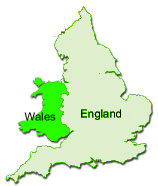
\includegraphics[width=0.45\columnwidth]{images/UK.png}
  \caption{Map of England and Wales}
  \label{fig:UK}
\end{figure}
\begin{figure}
  \centering
  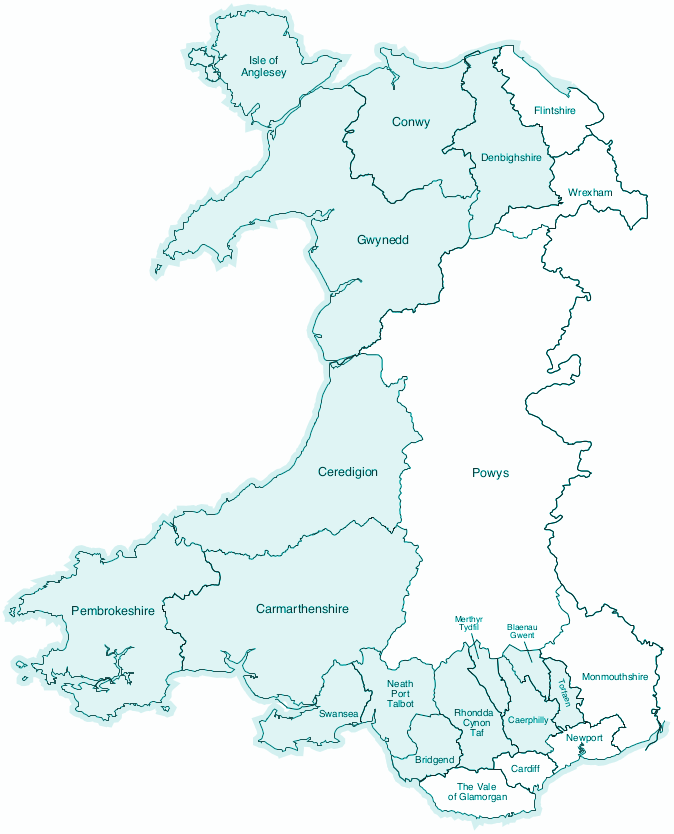
\includegraphics[width=0.45\columnwidth]{images/wales.png}
  \caption{Convergence region of Wales, consisting of 15 out of 22 regions}
  \label{fig:wales}
\end{figure}
carried out for Welsh Government estimates that
5\% of Welsh secondary students (ie, aged 11-19)
have engaged with Technocamps through Workshops,
and that more than a quarter of the secondary schools
in the region have established Technoclubs.

% taken from TOCE paper, can be adapted to Welsh focus
\section{Education in the UK}\label{sec:schools}

The UK consists of four nations ruled by one parliament:
England (population: 53.0 million), Scotland (5.3 million),
Wales (3.0 million) and Northern Ireland (1.8
million)\footnote{\url{http://www.ons.gov.uk/ons/guide-method/census/2011/index.html}}.
In 1997, Scotland and Wales held referendums which
determined in both cases the desire for self-government.
In the case of Wales, this led to the Government of Wales Act 1998
which created the National Assembly for Wales, to which
a variety of powers were devolved from the UK parliament
on 1 July 1999.
In particular,
education - which until then was a UK-wide government portfolio --
came under the control of the National Assembly for Wales,
under the direction of the Department for Education and Skills.

% % change this to have a brief discussion about all of the main
% systems in UK, especially England and Scotland (imp: Curric. for
% Excellence, plus Computing Science), then focus on Wales...

As noted in~\cite{Evans:2015},
the nation's education system
-- which was outperforming all other reguins in the UK
in the years prior to and immediately following devolution --
suffered a rapid decline.
Whilst maintaining the general educational system of Key Stages
used in England (See Figure~\ref{fig:key-stages}),
\begin{figure}
  \centering
  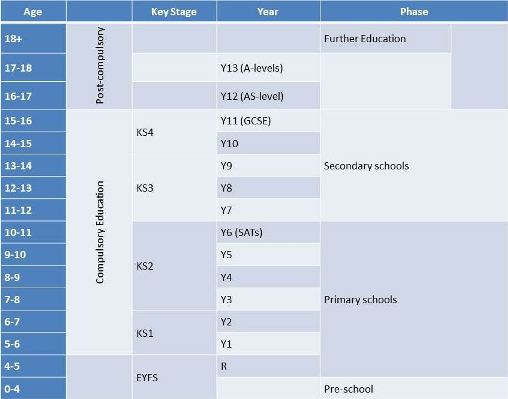
\includegraphics[width=\columnwidth]{images/keystages.png}
  \caption{Key Stages in the English and Welsh education system}
  \label{fig:key-stages}
\end{figure}
the Welsh Government embarked on a 10-year revolutionary plan
including
\begin{itemize}
\item
phasing out Standard Attainment Tests (SATs);
\item
replacing the early Key Stage 1 with
a play-based Foundation Phase;
\item
introducing the Welsh Baccalaureate at all levels:
an overarching qualification,
with a purely practical-based assessmen mechanism,
incorporating
key skills; Wales, Europe and the world;
work-related education; and personal and social education;
\item
focussing on the Welsh language and  Welsh-medium schools
\item
addressing the abundance of small schools in the 
predominantly rural communities throughout Wales.
\end{itemize}
Much of this plan was lauded, and time may yet prove its merits.
However, its implementation has been criticised
for various reasons and by various stakeholders;
and no fewer than 24 costly reviews have been commissioned
by the Department of Education and Skills
between June 2010 and February 2013 -- almost one per month.

With devolved autonomy comes autonomy over fiscal matters,
and the correlation between money and performance is
an obvious target for critics, who point to a growing spending shortfall 
between Wales and England.
The average spend per pupil in Wales in 2000-2001
-- just after devolution --
was more than every region of England apart from
the large metropolitan areas of London, the West Mindlans and the North West,
which all benefit from their economy of scale.
However, since then, the gap between
the education budgets per pupil between Wales and England
has steadily grown by about 1\% per year;
the figures forecast for 2013-2014 show
13\% more being spent per pupil in England than in Wales.

%As reported by Hubweiser et al.~\cite{hubwieser-et-al:2011}, when establishing
%a model for viewing school CS education, it is apparent that there is
%much diversity between school education systems, and this can create
%an obstacle when trying to understand progress made in a different
%country. Here we describe the context of school education in the UK.

% also: quals reform -- talk about WJEC and Wales in context of GCSEs
% and A-Levels!

%compulsory schooling until age 16.
%All subjects are
%compulsory until the end of Key Stage 3 (KS3) and then students can
%choose approximately ten subjects to study for the next two years,
%which each lead to GCSE (General Certificate of Secondary Education)
%qualifications. However, while the National Curriculum in England and
%Wales are broadly similar, they are distinct and use different
%terminology.

% adjust to be Wales-focused
%There is state provision for education in the UK up to the age of 19,
%with mostly comprehensive, mixed ability schools across the UK. A few
%areas in England have retained a system of selective 11+ schools
%called grammar schools, which require students to sit an exam prior to
%entry, but these schools are in the minority. As well as state
%schools, 10\% of schools in the UK are independent fee-paying
%schools. Overall, in England there are approximately 24,000 schools,
%including 16,800 primary schools, 3,400 secondary schools and 2,400
%independent schools (primary and secondary).  However, the primary and
%independent schools tend to be smaller: the state-funded schools had
%4.2 million primary pupils and 3.2 million secondary pupils, with 0.6
%million pupils in independent schools.

%The ICT curriculum in Wales
%(2008)\footnote{\url{http://wales.gov.uk/topics/educationandskills/schoolshome/curriculuminwales/arevisedcurriculumforwales/nationalcurriculum/ictnc/?lang=en}},
%was perceived to be less prescriptive than the ICT curriculum in
%England, but exhibiting many of the same issues. It was recently
%reviewed by an independent steering group appointed by the Welsh
%Government~\cite{welshictreview:2013}, making clear recommendations for
%reforming the ICT curriculum as part of a broader national curriculum
%review for September 2014.
%
% update end of this section so that it leads into the Donaldson review...

\subsection{ICT Curriculum Report 2013}

\textbf{Tom -- this is your story~\cite{welshictreview:2013};
Please write it.}

\subsection{Donaldson Report 2015}

\textbf{Tom -- please write this~\cite{Donaldson:2015}.}

\begin{quote}\it
In March 2014 Professor Graham Donaldson, a former chief school
inspector in Scotland, was asked to conduct an independent fundamental
review of curriculum and assessment arrangements of the entire
curriculum in Wales, from Foundation Phase to Key Stage 4.

Key points:

\begin{itemize}
\item structure of Foundation and Key Stages are going (moving away
  from the Ken Baker 1988 model!) -- unsurprisingly, feels quite
  similar to the Scottish Curriculum for Excellence model (link here);
\item replaced with six ``areas of learning'';
\item three cross-cutting "collective responsibilities": literacy, numeracy, digital competancies;
\item subjects should ``service the curriculum but not define it'';
\item lots of focus on creativity, as well as entrepreneurial activity;
\item big focus on citizenship, health and wellbeing (e.g. sex education, PSE);
\item assessment for learning, supporting excellence in learning and teaching;
\item Estyn need to change how they operate, promoting improvement not just testing'
\item Big hat-tip to the 2013 Review of the ICT curriculum, accepting
  importance of digital competancies, as well as computer science
  sitting within the new ``Science \& Technology'' area of learning.
\end{itemize}
\end{quote}

\subsection{Furlong Report 2015}

\textbf{Tom -- please write this~\cite{Furlong:2015}.}

\begin{quote}\it
Key points in the Furlong review of Initial teacher
education~\cite{Furlong:2015} (but not huge amounts of computing
specific stuff here) and the New Deal (ref, again not huge amounts of
specificity to computing education, but refer to QTS standards with
regards to expectations around digital competencies). Also refer to
incentivisation of entrants to the teaching profession (linking back
to ICT review~\cite{welshictreview:2013}), comparing
Wales\footnote{\url{http://teachertrainingcymru.org/node/16}}
vs. England\footnote{\url{https://getintoteaching.education.gov.uk/bursaries-and-funding}
and \url{http://academy.bcs.org/content/eligibility}}.
\end{quote}

\section{The Technocamps Effect}

Technocamps is a multi-faceted Universities-based
operation engaging with schools -- both their pupils and their teachers --
throughout Wales and across all ages. Its main activities are as follows.

\begin{description}
\item[Workshops]
One-day campus-based workshops offered to whole classes
to give the pupils an introduction to computing,
particularly computational thinking and problem solving.
The whole class approach allows us: to address the gender divide,
by engaging with an equal number of boys and girls;
and to engage with those with no predisposition (or indeed an aversion)
to digital technology, to create an interest of computing within them.
\item[Technoclubs]
Lunchtime clubs in schools where pupils develop
their computational thinking and building skills.
\item[Bootcamps]
Two-day campus-based workshops held during school holidays.
\item[After Schools Clubs]
Two-hour late afternoon sessions held on campus or in the community.
\item[Playground Computing]
Day-long in-school workshops which present
the fundamentals of computer science to primary school pupils
through playful activities which develop computational thinking
and problem solving skills, but do not involve computers.
\item[Technoteach]
Training sessions, typically in the form of 20-hour modules
delivered one evening per week over six weeks.
Technoteach also encompasses other standalone twilight sessions
as well as an annual teachers conference.
\item[NEET Engagement]
Week-long summer residential sessions run in partnership with
the municipal youth services in which young people identified
as NEET (Not in Employment, Education of Training)
carry out a variety of team-building exercises,
learn app development and compete to design and build the best app.
\item[Student Placements]
Computer Science students at the University are offered
the opportunity to gain university course credits through
placements -- one day per week -- as teaching assistants
in school computing/ICT classes.
\end{description}

All Technocamps activities are provided completely free of charge
for all of its participants. This represents a huge investment
on the part of the Universities, but Technocamps has also received
various sources of funding in support of its activities.
The main funders are as follows.
\begin{description}
\item[ESF] (October 2010 - September 2014) --
A four-year \pounds 6 million EU-funded project to engage with secondary schools across South West Wales and the Valleys. This project involved Technocamps hubs at Aberystwyth University, Bangor University and the University of South Wales Glamorgan. Some 9,000 pupils from more than 180 schools and colleges have benefited from this project, as well as their teachers.
\item[NESTA] (June 2013 - December 2014) --
An 18-month \pounds 46,000 project to support the Playground Computing programme. This funding allows for a teacher to be seconded for 18 months to Technocamps in order to go out to primary schools throughout South Wales every day to present workshops. It has seen some 5,000 pupils at over 50 primary schools enjoy multiple day-long visits.
\item[National Science Academy] (November 2013 - March 2015) --
A 17-month \pounds 24,000 project to support the Technoteach programme; this funding was mainly in support of teachers registering on our six-week Technoteach modules, specifically providing their schools an amount of teacher cover to facilitate their attendance on the module. Over 120 teachers have thus far benefited from this project.
\item[Welsh Government] (September 2014 - March 2016) --
An 18-month \pounds 370,000 project under the Welsh Government's Learning in Digital Wales (LiDW) Tender. The LiDW Tender is to deliver 3-hour taster sessions at each of the 210 state-sponsored secondary schools across Wales, and will be delivered by each of the six Technocamps hubs.
\end{description}

\section{Conclusions}
What are the top-line messages???
% data from ICT review survey?

% bib
\bibliographystyle{abbrv}
\bibliography{wipsce2015}

%\section*{To Do}
%
%In no particular order...
%
%\begin{itemize}
%\item Set UK context over past 3-5 years
%\item Link to English and Scottish changes
%\item Welsh context
%\item Technocamps: the ten year journey from 2003
%\item Convergence, the pan-Wales problem
%\item Key contributions: aims, targets, impacts, young people, NEETs, coverage
%\item Links with CAS Wales
%\item Hubs (both TC and CAS)
%\item Funding models: ESF, NSA, Nesta, etc
%\item {\textbf{Key theme}}: Building capacity, the problems of
%  England's NoE model in Wales
%\item UK policy: RS report, English curriculum, qualification change,
%  UKForCE, etc.
%\item Welsh policy: ICT curriculum, ICT review, Estyn reports, ICT
%  sector support/economic drivers, curriculum change,
%  Donaldson and post-Donaldson
%\item THE FUTURE...!
%\end{itemize}
%
%\subsection*{References to fit in}
%\begin{itemize}
%\item
%General CAS
%citations~\cite{crick+sentance:2011,brown-et-al-sigcse2012,brown-et-al-toce2014}.
%
%\item
%Teachers, CPD and
%NoE~\cite{sentance-et-al-wipsce2012,sentance-et-al:2013,sentance-et-al:2014}.
%
%\item
%Technocamps~\cite{ball-et-al:2012,boyle-et-al:2012}
%
%\item
%Welsh Government report:
%\begin{itemize}
%\item
%ICT Review~\cite{welshictreview:2013}
%\item
%Graham Report on STEM~\cite{STEMreview:2014}
%\item
%Donaldson Report~\cite{Donaldson:2015}
%\item
%Furlong Report~\cite{Furlong:2015}
%\end{itemize}
%
%\item
%Misc Reports
%\begin{itemize}
%\item
%NESTA Report~\cite{NESTA:2015}
%
%\end{itemize}
%\end{itemize}

\end{document}
